\chapter{Testing}

	\section{Unit testing}
		Per tutti i test viene supposto che le stringhe da cifrare siano state processate dal parser e quindi che contengano solamente caratteri effettivamente cifrabili. Per eliminare tale dipendenza da classi concrete, nei vari unit-test un'istanza del parser viene simulata tramite \emph{mocking} e \emph{stubbing} dei metodi. Tale metodo verrà approfondito più avanti.
		
		Andiamo a vedere nel dettaglio i test con i quali sono state implementate le varie classi.
		
		\subsection{Shift cipher}
			Lo \emph{shift cipher} è il cifrario più semplice. L'unica cosa che fa è spostare la lettere da cifrare di un certo numero di posizioni avanti nell'alfabeto. Tale numero di posizioni è la chiave del cifrario. Per decifrare il messaggio basterà semplicemente tornare indietro del numero di posizioni indicato dalla chiave. Se per esempio il messaggio è \emph{ciao} e la chiave è 3, il messaggio cifrato sarà \emph{fldr}.
			
			Le uniche due funzionalità richieste a questo cifrario sono quelle di cifratura e decifratura. Tali funzionalità sono state testate nel caso di uno spostamento di zero posizioni (non ottenendo una cifratura), di una posizione, di ventisei posizioni, di ventisette posizioni e di un numero negativo di posizioni(-1). Come caso limite è stata testata anche la cifratura della stringa vuota (il numero di posizioni è ininfluente dato che la cifratura terminerà immediatamente).
			
			Testando anche la decifratura di tutti questi casi sono state coperte le possibili modalità di cifratura/decifratura di una stringa.
			
		\subsection{Affine cipher}
			L'Affine cipher è una generalizzazione dello shift cipher. Questo cifrario ha come chiave due parametri \emph{a} e \emph{b} opportunamente scelti secondo principi di algebra modulare. La i-esima lettera P[i] del messaggio in chiaro verrà cifrata in (P[i] * \emph{a} + \emph{b}) modulo 26. Se viene scelto il parametro \emph{a} = 1 otteniamo in tutto e per tutto uno shift cipher.
			
			I comportamenti da testare sono la cifratura, la decifratura e la giusta scelta del  parametro \emph{a} che deve essere coprimo con 26.
			
			Questo ultimo comportamento viene testato dando in input 2 come coefficiente \emph{a} e aspettandosi una IllegalArgumentException.
			
			La cifratura e la decifratura vengono testate con stringhe di lunghezza variabile per cercare di coprire il maggior numero di combinazioni possibili.
			
		\subsection{Vigenere cipher}
			Il \emph{cifrario di Vigenère} è un'altra variante dello shift cipher che invece di utilizzare come chiave un numero fisso, utilizza una parola che viene ripetuta tante volte fino al raggiungimento della lunghezza del messaggio che si vuole cifrare. Ogni lettera verrà poi traslata del numero di posizioni corrispondenti alla posizione nell'alfabeto della corrispondente lettera della chiave.
			
			Se per esempio abbiamo un certo messaggio P da cifrare con una chiave K, allora come prima cosa verrà ripetuta K tante volte fino a che la sua lunghezza non raggiunge quella di P e poi ogni i-esima lettera P[i] del messaggio sarà cifrata in P[i]+K[i] modulo 26.
			
			Cifrare il messaggio \emph{testmessage} con la chiave \emph{test} comporterà tre ripetizioni della chiave (che quindi diventerà \emph{testtesttest}). Conseguentemente la prima lettera del messaggio (\emph{t}) verrà spostata di venti posizioni (verrà cifrata con la prima lettera della chiave che è \emph{t} ed è la ventesima lettera dell'alfabeto), la seconda di cinque e così via.
			
			I comportamenti da testare sono la cifratura, la decifratura e il prolungamento della chiave.
			
			Cifratura e decifratura sono testati con stringhe di lunghezze diverse, sempre per coprire il maggior numero di combinazioni possibili.
			
			L'estensione della chiave viene testata fornendo la stringa \emph{test} come chiave, facendo cifrare il messaggio \emph{testmessage} e verificando che sia stata trasformata in \emph{testtesttest}.
			
			Sono presenti anche tre test che controllano l'inserimento di una chiave illegale. Questi test sono stati inseriti per chiarire meglio il comportamento di questa classe ma sarebbero inutili in quanto questo controllo viene in realtà fatto dal parser.
			
		\subsection{OneTimePad cipher}
			Il cifrario OneTimePad è una specializzazione del cifrario di Vigenère che richiede come chiave una stringa binaria della lunghezza almeno pari alla conversione in stringa binaria del messaggio da cifrare. Questo cifrario viene anche chiamato \emph{cifrario perfetto} ed è l'unico sistema crittografico la cui sicurezza sia comprovata da una dimostrazione matematica nel 1949 da \emph{Claude Shannon}.
			
			Questo cifrario è un po' più complesso dei precedenti in quanto prevede una conversione del messaggio da cifrare in una stringa binaria. Una volta convertita il messaggio cifrato si otterrà semplicemente operando uno XOR tra le due stringhe binarie.
			
			I comportamenti da testare sono quindi molteplici.
			
			Il primo comportamento testato è quello di creazione della chiave (che avviene con un generatore casuale). Questo comportamento viene testato confrontando la lunghezza della stringa data in input e la lunghezza della chiave restituita.
			
			Successivamente viene testata la capacità di convertire un messaggio nella relativa stringa binaria. Per questa conversione viene utilizzata la codifica di Huffmann dell'alfabeto inglese.
			
			Viene testata anche l'operazione inversa, cioè quella di riconvertire una stringa binaria ottenuta dalla codifica precedente in una stringa di testo. Questo permetterà di ottenere un messaggio decifrato leggibile.
			
			Come ultima cosa, vengono testate la cifratura e la decifratura.
			
			Tutti questi controlli, come per i casi precedenti, vengono ripetuti su stringhe di lunghezza differente per coprire ogni caso possibile.
			
		\subsection{Substitution cipher}
			Anche il substitution cipher è un cifrario abbastanza semplice che utilizza come chiave di cifratura una permutazione dell'alfabeto. Se per esempio la permutazione utilizzata è \emph{qwertyuiopasdfghjklzxcvbnm} la lettera \emph{a} verrà sostituita con la \emph{q}, la \emph{b} con la \emph{w} e così via fino a scambiare la \emph{z} con la \emph{m}.
			
			I comportamenti importanti da testare per questo cifrario sono ovviamente la cifratura e la decifratura ma anche il corretto settaggio della permutazione dell'alfabeto da utilizzare come chiave.
			
			Cifratura e decifratura vengono testate con stringhe lunghe zero (stringa vuota), uno e quattro caratteri (questa scelta è dovuta solamente per cercare la cifratura di una stringa di senso compiuto, in questo caso \emph{test}). La permutazione utilizzata è appunto quella specificata nell'esempio iniziale.
			
			Come prima, i test riguardanti il controllo della permutazione di cifratura in realtà non sarebbero necessari in quanto già presenti nei test del parser (che è quello che si occupa di questo controllo) ma sono stati aggiunti per specificare meglio il comportamento che deve avere la classe in caso di inserimento di una permutazione scorretta (troppo corta, troppo lunga o con caratteri non alfabetici).
			
		\subsection{InputManager}
			Questa è la classe concreta che implementa l'interfaccia \emph{Parser}. Il suo scopo è gestire le varie stringhe passate ai cifrari restituendo solamente caratteri cifrabili.
			
			Il metodo \emph{process} riceve come parametro una stringa, rimuove tutti i caratteri che non sono lettere e converte tutte le lettere maiuscole in minuscole.Questo metodo viene testato passando come argomento una stringa già nella forma voluta, una con un carattere non alfabetico, una con uno spazio, una con delle maiuscole e una vuota.
			
			Il metodo \emph{checkAlphabet} riceve sempre una stringa come parametro e controlla che sia formata da esattamente ventisei lettere. Se sono meno, più o sono presenti caratteri non alfabetici restituisce un'eccezione.Anche questo metodo viene testato cercando di simulare ogni possibile input quindi con una stringa corretta, una più corta, una più lunga, una con un carattere non alfabetico e una con lettere maiuscole (che non solleva eccezione).
			
			Il metodo \emph{checkKey} riceve una stringa e un intero \emph{l} e si occupa di verificare che la stringa ricevuta sia una stringa binaria di lunghezza \emph{l}. Questo metodo viene testato prima passando una stringa binaria e la lunghezza corrispondente e poi aspettandosi un'eccezione quando gli vengono passate prima una stringa contenente un carattere diverso da 0 o 1 e successivamente un intero maggiore della lunghezza della stringa.
			
		\subsection{Constants}
			In questa classe vengono semplicemente definite delle costanti condivise tra tutte le classi del programma. Essendo tutti campi \emph{static} l'unico comportamento da testare è l'impossibilità di creare un nuovo oggetto di questo tipo.
			
			Il primo test si occupa di verificare che il costruttore sia effettivamente privato utilizzando le reflection di Java attraverso il metodo isPrivate.
			
			Il secondo controlla appunto che una eventuale creazione di un oggetto di tipo \emph{Constants} restitutisca una UnsupportedOperationException.
			
	\section{Mocking}
		Per eliminare la dipendenza da altre classi concrete che potrebbero disturbare lo unit-testing, nelle cinque classi che implementano i cifrari, viene utilizzato un \emph{mock} dell'interfaccia parser.	Ognuna di queste cinque classi utilizza infatti un oggetto di questo tipo per effettuare vari controlli sulle stringhe fornite in input.
		
		Lo stubbing dei metodi usati da vari test-case viene effettuato direttamente nel metodo setup annotato come \emph{@Before} mentre quelli usati solamente da un singolo test-case vengono effettuati all'interno del relativo test-case.
		
	\section{Mutation testing}
		Per il mutation testing è stato utilizzato PIT. Sono stati attivati gli strong mutator e il risultato del testing è visibile in figura \ref{fig:pit}
		
		\begin{figure}[h]
			\centering
			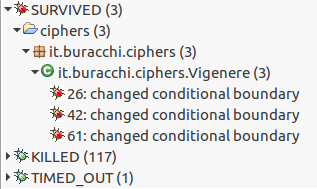
\includegraphics[scale=0.5]{img/PIT}
			\caption{Risultati del mutation testing}
			\label{fig:pit}
		\end{figure}
		
		Dei 121 mutanti creati solamente tre sopravvivono. Questo però non viene ritenuto un problema perché i mutanti sopravvissuti non compromettono la funzionalità del programma. Il comportamento mutato è infatti il controllo del fatto che la lunghezza della chiave nel cifrario di Vigenère sia almeno quanto la lunghezza del messaggio che si vuole cifrare. Nel codice è stato utilizzato un < ma ovviamente, visto che la lunghezza della chiave non deve necessariamente essere uguale a quella del messaggio ma può essere superiore, cambiare questo controllo con un <= non cambia la funzionalità del metodo e non deve neanche generare un errore.
		
		L'unico effetto riscontrato sarà un prolungamento inutile della chiave che però non porta alcun problema.
		
	\section{Integration testing}